\chapter{Evaluation}
\label{chapter:evaluation}
\thispagestyle{myheadings}

% set this to the location of the figures for this chapter. it may
% also want to be ../Figures/2_Body/ or something. make sure that
% it has a trailing directory separator (i.e., '/')!
\graphicspath{{./5_Evaluation/}}
\section{Optimality checking}
Now we have learnt a model $Q_{\theta}$, we also have our test cases $\{(x_{i},y_{i})\}_{i\in[n]}$.\\
Each data window corresponds to $24$ data entries. The $t^{th}$ window corresponds to 
$$\{x_{24t}, x_{24t+1}, ..., x_{24t+23}|t\in\mathbb{I}\}$$
Each data window has $24$ data points as we have tried all possible($24$ of them) combinations of ordering of operations. For each data window we need to find the ordering of operations which requires the minimum moves according to our predictions.\\
To do this for the $t^{th}$ window of data, find the index of the minimum of $$Q_{\theta}(x_{24t}),Q_{\theta}(x_{24t+1}),...,Q_{\theta}(x_{24t+23})$$, say $k$.\\
To check if the move this corresponds to is the actual optimal move, find the index of the minimum of $y_{24t}, y_{24t+1}, ..., y_{24t+23}$, say $l$. If $k=l$ then the move we predicted as optimal is indeed optimal.\\ 
\par We train the model multiple times on the training data and measure its performance on the test data each time.\\
To measure the performance we use the predicted optimal move vs the actual optimal move.\\

\section{Justification}
The things considered while determining the neural network to use for training the DQN are :-
\begin{itemize}
    \item To achieve a value as close as possible to the global minima for the optimization function (Adam optimzer)
    \item The time required to predict the optimal move should not exceed the time saved by using it.
    \item The time and resources required for training should not exceed the capacity of the system while it is running the query processing in the background. 
\end{itemize}
What we found was:-
\begin{itemize}
    \item Adding additional layers improve the prediction of the optimal moves but not by significant margin.
    \item Adding additional layers resulted in the time spent predicting the answer overshadowing the time saved by executing the optimal move.
\end{itemize}
\par But note, these $2$ are only query and data specific findings.

\section{Results}
First, for each ordering of the operations we present the frequencies with which they are optimal in the dataset.
\begin{lstlisting}[caption=Frequencies of optimal moves in total data]
[0, 0, 0, 0, 0, 0, 0, 0, 0, 1, 0, 0, 110, 83, 84, 79, 80, 63, 307, 165, 2209, 1367, 43849, 43872]
\end{lstlisting} 
As visible the data is higly biased towards the last $2$ orderings.\\
We split this data into $70\%,30\%$ for the purpose of training and testing of our reinforcement learning agent.The random seed used resulted in the following split.
\begin{lstlisting}[caption= Frequencies of optimal move in training data]
[0, 0, 0, 0, 0, 0, 0, 0, 0, 0, 0, 0, 81, 60, 59, 54, 57, 45, 227, 119, 1526, 966, 30811, 30583]
\end{lstlisting}
\begin{lstlisting}[caption= Frequencies of optimal move in testing data]
[0, 0, 0, 0, 0, 0, 0, 0, 0, 1, 0, 0, 29, 23, 25, 25, 23, 18, 80, 46, 683, 401, 13038, 13289]
\end{lstlisting}
The predictions of our model resulted in the following $24$ true positive, False Positive, False negative and True negative results\\
\begin{lstlisting}[caption= True positives False positives False negatives True negatives]
(TP,FP,FN,TN)
(0.0, 0.0, 0.0, 27681.0)
(0.0, 0.0, 0.0, 27681.0)
(0.0, 0.0, 0.0, 27681.0)
(0.0, 0.0, 0.0, 27681.0)
(0.0, 0.0, 0.0, 27681.0)
(0.0, 0.0, 0.0, 27681.0)
(0.0, 0.0, 0.0, 27681.0)
(0.0, 0.0, 0.0, 27681.0)
(0.0, 0.0, 0.0, 27681.0)
(0.0, 0.0, 1.0, 27680.0)
(0.0, 0.0, 0.0, 27681.0)
(0.0, 0.0, 0.0, 27681.0)
(0.0, 0.0, 29.0, 27652.0)
(0.0, 3.0, 23.0, 27655.0)
(0.0, 0.0, 25.0, 27656.0)
(0.0, 0.0, 25.0, 27656.0)
(0.0, 0.0, 23.0, 27658.0)
(0.0, 0.0, 18.0, 27663.0)
(0.0, 7.0, 80.0, 27594.0)
(0.0, 0.0, 46.0, 27635.0)
(18.0, 251.0, 665.0, 26747.0)
(69.0, 973.0, 332.0, 26307.0)
(6347.0, 6789.0, 6691.0, 7854.0)
(6355.0, 6869.0, 6934.0, 7523.0)
\end{lstlisting}
So we got $12978$ predictions correct out of $27681$ test cases that is around $47\%$.
Below are 2 confusion matrices we obtained from two different runs of the predictions.\\

\begin{figure}
\caption{DQN Run 1 confusion matrix}
\centering
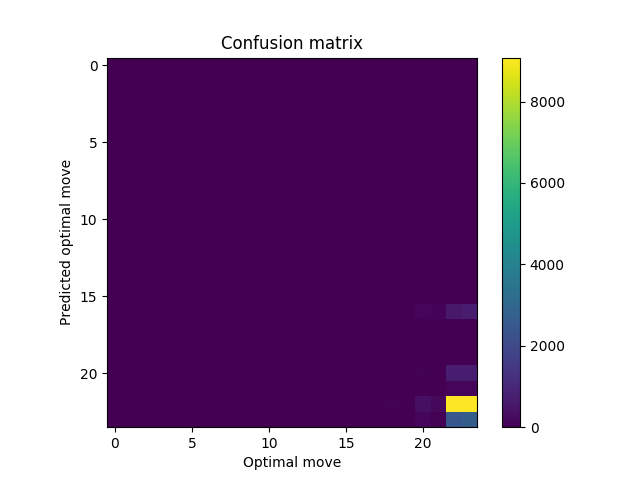
\includegraphics[scale=1]{cm1.png}\\
\end{figure}

\begin{figure}
\caption{DQN Run 1 confusion matrix closeup}
\centering
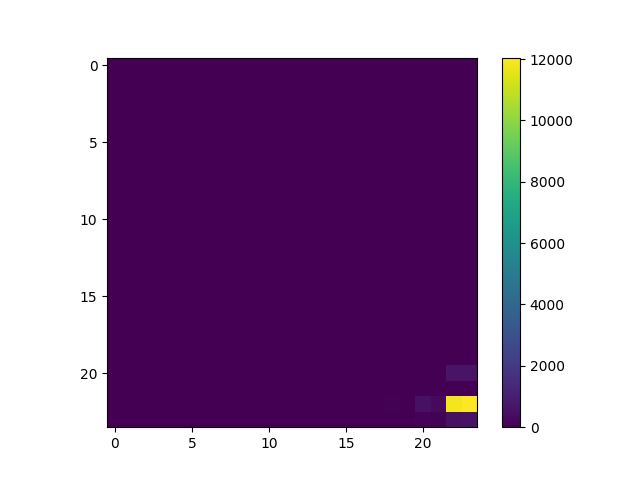
\includegraphics[scale=1]{cm2.png}\\
\end{figure}

\begin{figure}
\caption{DQN Run 2 confusion matrix}
\centering
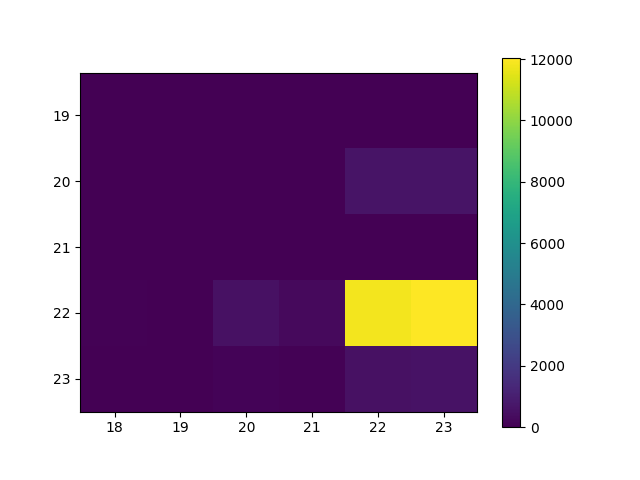
\includegraphics[scale=0.5]{cm3.png}\\
\end{figure}

\begin{figure}
\caption{DQN Run 2 confusion matrix closeup}
\centering
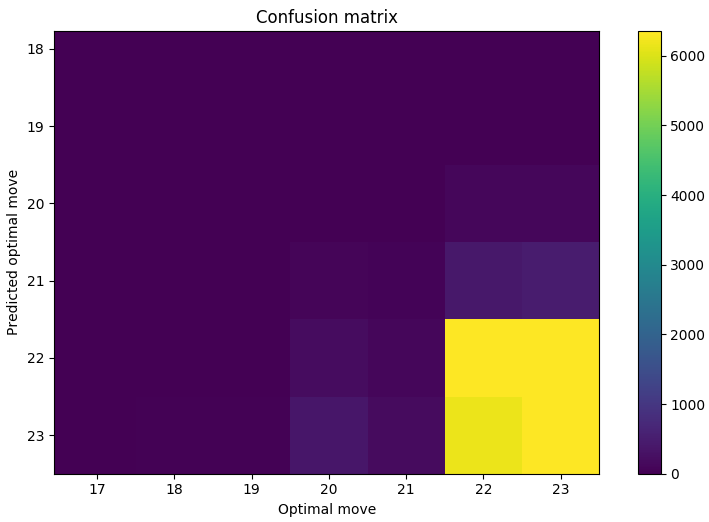
\includegraphics[scale=0.5]{cm4.png}\\
\end{figure}

Also have the actual confusion matrix for the second run.\\
\begin{lstlisting}[caption=Confusion matrix for DQN classificaiton]
[[   0    0    0    0    0    0    0    0    0    0    0    1    0]
 [   0    0    0    0    0    0    0    0    0    0    0   16   13]
 [   0    0    0    0    0    0    0    0    0    0    0   18    5]
 [   0    0    0    0    0    0    0    0    0    0    0   13   12]
 [   0    0    0    0    0    0    0    0    0    0    0   12   13]
 [   0    0    0    0    0    0    0    0    0    0    0   17    6]
 [   0    0    0    0    0    0    0    0    0    0    0    9    9]
 [   0    0    0    0    0    0    0    0    0    0   10   21   49]
 [   0    0    0    0    0    0    0    0    0    3    4   13   26]
 [   0    0    0    0    0    0    0    1    0   18   77  213  374]
 [   0    0    0    0    0    0    0    0    0   19   69  118  195]
 [   0    0    2    0    0    0    0    0    0  116  406 6347 6167]
 [   0    0    1    0    0    0    0    6    0  113  476 6338 6355]]
\end{lstlisting}
We have the actual optimal ordering, the actual worst ordering, the predicted best ordering from the model.\\
We add the number of operations required by following each of the above $3$ and look at the sum of them.\\
\begin{itemize}
    \item The sum of operations required by the optimal ordering $890640075.0$
    \item The sum of operations required by the predicted ordering $900269878.0$
    \item The sum of operations required by the optimal ordering $2310227856.0$
\end{itemize}
This tells us that our predicted orderings are approx $39\%$ of the worst ordering and $102\%$ of the best ordering.\\
A label based analysis is obtained by using $"\text{metrics.classification\_report}"$ from \\
 scikit-learn\cite{scikit-learn}.\\
\begin{lstlisting}[caption=Statistics for various orderings]
             precision    recall  f1-score   support

           9      0.000     0.000     0.000         1
          12      0.000     0.000     0.000        29
          13      0.000     0.000     0.000        23
          14      0.000     0.000     0.000        25
          15      0.000     0.000     0.000        25
          16      0.000     0.000     0.000        23
          17      0.000     0.000     0.000        18
          18      0.000     0.000     0.000        80
          19      0.000     0.000     0.000        46
          20      0.067     0.026     0.038       683
          21      0.066     0.172     0.096       401
          22      0.483     0.487     0.485     13038
          23      0.481     0.478     0.479     13289

   micro avg      0.462     0.462     0.462     27681
   macro avg      0.084     0.089     0.084     27681
weighted avg      0.461     0.462     0.461     27681
\end{lstlisting}

\section{Discussion}

\section{Conclusion}
In this chapter we saw :-
\begin{itemize}
    \item The method for selecting the optimal move and the assumption for it.
    \item The classificaiton of the data and how it is split between training and testing.
    \item Analyzed and visualized the confusion matrix on different runs of DQN.
    \item The performance of the DQN on predicting.
\end{itemize}
In the next chapter we:-
\begin{itemize}
    \item Present the overall results of the thesis.
    \item Present the take aways.
    \item Present the ways of improving upon this work.
\end{itemize}
%1.2 change to research problem. Most important, 1.4
%Explain and justify reinforcement learning
%What we have seen in thsi chapter, what we will see in next chapter
%Typing error, grammar
